\documentclass{article}
\usepackage{overture}
\usepackage{fullpage}
\usepackage{longtable}
\usepackage{alltt}
\usepackage{graphicx}
\usepackage{makeidx}
\makeindex

\title{VDM++ Sorting Algorithms}
\author{Peter Gorm Larsen}

\begin{document}
\maketitle

\section{Introduction}

This document contains a sorting example. The class diagram can be
seen in Figure \ref{inh}.  The structure of the example is known as
the \textit{strategy} pattern. This pattern defines a family of
algorithms, encapsulates each one and make them interchangeable. The
\textit{strategy} pattern lets the algorithm vary independently from
clients that use it. The \texttt{SortMachine} class is the client that uses the
different sorting algorithms. The \texttt{Sorter} class is an abstract class
that defines a common interface to all supported algorithms.


\begin{figure}[tbh]
\begin{center}
\mbox{}
\resizebox{12cm}{!}{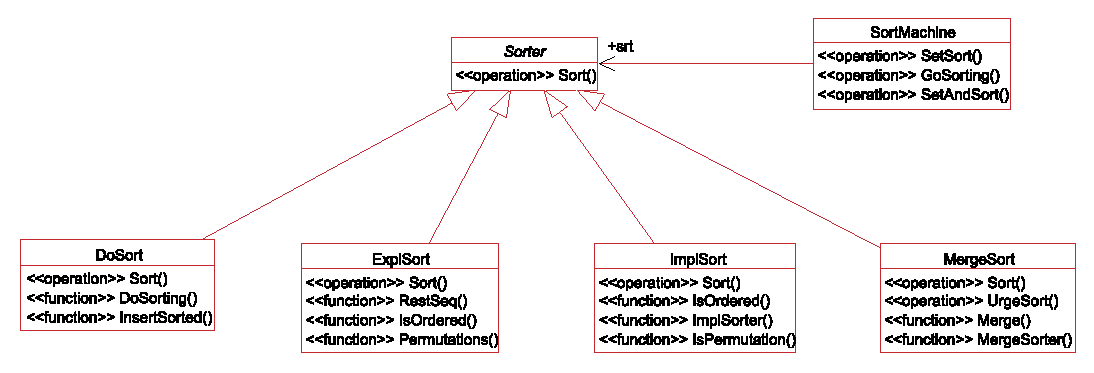
\includegraphics{../../inherit2}}
\caption{Class diagram for the sort example}\label{inh}
\end{center}
\end{figure}

\input{specification/sortmachine.vdmpp.tex}

\input{specification/sorter.vdmpp.tex}

\input{specification/mergesort.vdmpp.tex}

\input{specification/dosort.vdmpp.tex}

\input{specification/implsort.vdmpp.tex}

\input{specification/explsort.vdmpp.tex}

\newpage
\addcontentsline{toc}{section}{Index}
\printindex

\end{document}
